%\section{Exponential Generating Functions}
\begin{python0}
from solutions import *; clear() 
\end{python0}

If you look at all the above examples involving generating functions, 
you notice that they all involve selecting objects.
What if you're interested in selecting \textit{and} permuting
objects -- i.e. order is important.

Now if $a_n$ is the number of ways to select $n$ objects from a pool
under some constraint, why do we use $\sum_{n=0}^\infty a_n x^n$
as the generating function?
Why not $\sum_{n=0}^\infty a_n \sin(nx)$?

Because if $b_n$ is the number of ways to select from another set
then 
\[
\sum_{n=0}^\infty a_n x^n \cdot \sum_{n=0}^\infty b_n x^n
= \sum_{n=0}^\infty (a_0b_n + \cdot + a_n b_0) x^n
\]
gives the generating function for selecting $n$ objects from both sets.

Now let's go back to permutations.

Suppose $a_n$ is the number of ways to select $n$ objects (under some
constraint). 
Then the number of ways to select $n$ objects and to permute the objects
is
\[
n! a_n
\]
(right?)
The function $\sum_{n=0}^\infty a_n x^n$ can be written as
\[
\sum_{n=0}^\infty (n!a_n) \frac{x^n}{n!}
\]
In general, if $b_0, b_1, b_2, \cdots$ is a sequence of numbers, then the 
\defone{exponential generating function} of $b_0, b_1, b_2, \ldots$is 
\[
\sum_{n=0}^\infty b_n \frac{x^n}{n!}
\]
(More generally, if you have a bunch of functions written
$K_n(x)$, you can form generating functions
$\sum_{n=0}^\infty a_n K_n(x)$.
Up to this point we've considered $K_n(x) = x^n$ for
ordinary generating functions and $K_n(x) = x^n/n!$ for 
exponential generating functions.)

Does multiplication work for exponential generating functions?
Let 
$a = \sum_{n=0}^\infty a_n \frac{x^n}{n!}$ 
and 
$b = \sum_{n=0}^\infty b_n \frac{x^n}{n!}$ 
be exponential generating functions where
$a_n$ is the number of ways of selecting $n$ objects from the a first set
and permutating them
and 
$b_n$ is the number of ways of selecting and permutating $n$ 
objects from a second pool.
Consider the product of the $i$--th term from $a$ and $j$--th term
from $b$, i.e. the product 
\[
a_i \frac{x^i}{i!} \cdot
b_j \frac{x^j}{j!}
\]
We have
\begin{align*}
a_i \frac{x^i}{i!} \cdot b_j \frac{x^j}{j!}
&= \frac{a_i}{i!} \cdot \frac{b_j}{j!}  \cdot x^{i+j}
\end{align*}
Not very helpful!
But if I rewrite the above like this:
\begin{align*}
a_i \frac{x^i}{i!} \cdot b_j \frac{x^j}{j!}
&= a_i \cdot b_j \cdot  \frac{(i+j)!}{i! j!} 
\cdot \frac{x^{i+j}}{(i+j)!} \\
\end{align*}
you see that the coefficient in front of $x^{i+j}/(i+j)!$ is
\[
\frac{a_i}{i!} \cdot \frac{b_j}{j!} \cdot (i+j)! 
\]
which is the number of ways of selecting $i$ objects from the first pool,
followed by the number of ways of selecting $j$ objects from the 
second pool, followed by permutating $i + j$ objects.
(if $a_i$ is the number of ways to select $i$ objects
and permutating them, then $a_i/i!$ is the number of ways
to select $i$ objects -- see earlier remarks.)

Therefore, on multiplying the two series, we have
\begin{align*}
a \cdot b 
&= \sum_{n=0}^\infty a_n \frac{x^n}{n!} \cdot 
   \sum_{n=0}^\infty b_n \frac{x^n}{n!} \\
&= \sum_{n=0}^\infty
\biggl(
\frac{a_0 b_n}{0! n!} (0+n)! \frac{x^{0+n}}{(0+n)!} \\
&\hskip 1cm + \frac{a_1 b_{n-1}}{1! (n-1)!} (1+(n-1))! \frac{x^{1+(n-1)}}{(1+(n-1))!} \\
&\hskip 1cm + \cdots \\
&\hskip 1cm + \frac{a_n b_0}{n! 0!}(n+0)!\frac{x^{n+0}}{(n+0)!}
\biggr) \\
&= \sum_{n=0}^\infty
\biggl(
\frac{a_0 b_n}{0! n!} +
\frac{a_1 b_{n-1}}{1! (n-1)!} +
\cdots +
\frac{a_n b_0}{n! 0!}
\biggr) n! \cdot \frac{x^n}{n!}
\end{align*}
The coefficient of $x^n/n!$ is the number of ways of 
$0$ object from the first pool and $n$ objects from the second pool
and permuting them, or
$1$ object from the first pool and $n-1$ objects from the second pool
and permuting them, or ...
which is the same as the number of ways of 
selecting $n$ objects from the first and second pool and permuting them.

Note that while the \lq\lq basic'' (ordinary) generating function 
for $1, 1, 1, \ldots$ is
\[
\sum_{n=0} 1 \cdot x^n = \sum_{n=0}^\infty x^n = \frac{1}{1-x}
\]
the exponential generating function for $1, 1, 1, \ldots$ is
\[
\sum_{n=0} 1 \cdot \frac{x^n}{n!} = 
\sum_{n=0}^\infty \frac{x^n}{n!} = e^x
\]
Therefore, whereas mathematical tools/formulas for rational functions 
are crucial in order to work effectively with ordinary generating functions,
for the case of 
exponential functions, we must know how to handle 
exponential functions well. 

[facts on and related to $e^x$, etc.]

\begin{eg}
How many ways are there to arrange 4 letters in ENGINE?
\end{eg}

Now the word \lq\lq arrange'' means that order does mattter.
So don't use ordinary generating functions!

First let's think about the exponential generating function for 
selecting and Es. 
\begin{align*}
\text{number of ways to select 0 E's and permute them} &= 1 \\
\text{number of ways to select 1 E's and permute them} &= 1 \\
\text{number of ways to select 2 E's and permute them} &= 1 \\
\text{number of ways to select 3 E's and permute them} &= 0 \\
\text{number of ways to select 4 E's and permute them} &= 0 \\
... &
\end{align*}
Therefore the exponential generating function, say $E$, is
\[
E = 
1 \frac{x^0}{0!} +
1 \frac{x^1}{1!} +
1 \frac{x^2}{2!} +
0 \frac{x^3}{3!} +
0 \frac{x^3}{4!} +
\cdots
= 1 + x + \frac{x^2}{2!}
\]
Write $N$, $G$, and $I$
for the exponential generating function for selecting
and permuting N's, G's, and I's respectively.
Then
\begin{align*}
N &= 1 + x + \frac{x^2}{2!}\\
G &= 1 + x \\
I &= 1 + x\\
\end{align*}
Altogether the required number must be coefficient of $x^4/4!$
of $ENGI$.
Let's compute that:
\begin{align*}
ENGI
&= 
\biggl( 1 + x + \frac{x^2}{2!} \biggr)^2
(1+x) \\
&= 1 + x + 4x + 7x^2 + 7x^3 + \frac{17}{4}x^4
+ \frac{3}{2}x^5
+ \frac{1}{4}x^6
\end{align*}
Now watchout! 
The coefficient of $x^4$ is $17/4$.
The coefficient we want is the coefficient of 
$x^4/4!$.
The term containing $x^4$ is
\[
\frac{17}{4} x^4 =
\frac{17}{4} 4! \cdot \frac{x^4}{4!}
\]
Hence the required number is
\[
\frac{17}{4} 4!
\]
or $17 \cdot 3!$.




\begin{eg}
How many arrangements of 12 symbols are there out of 12 R's, 12 W's, 12 B's,
12 C's. if

(a) We have an even number of B's, odd number of C's.

(b) We have at least 3 W's or no W's
\end{eg}

(a) The exponential generating function is
\[
f(x) = \biggl( 1 + x + \frac{x^2}{2!} + \cdots \biggr)^2
\cdot 
\biggl( 1 + \frac{x^2}{2!} +  \frac{x^4}{4!} \cdots \biggr)
\cdot 
\biggl( x + \frac{x^3}{3!} +  \frac{x^5}{5!} \cdots \biggr)^2
\]
Recall that
\[
e^x 
= 1 + x + \frac{x^2}{2!} + \cdots  
= \sum_{n=0}^\infty \frac{x^n}{n!}
\]
Now watch the following tricks.
First of all from the above power series for $e^x$,
on replacing $x$ with $-x$ we get
\[
e^{-x} = 
= 1 - x + \frac{x^2}{2!} - \cdots  
= \sum_{n=0}^\infty \frac{(-x)^n}{n!}
= \sum_{n=0}^\infty (-1)^n \frac{x^n}{n!}
\]
On adding the power series of $e^x$ and $e^{-x}$ we get
\begin{align*}
e^x + e^{-x} 
&= 2 + 2 \frac{x^2}{2!} + 2 \frac{x^4}{4!} + 2 \frac{x^6}{6!} + \cdots \\
&= 2 \biggl( 
   1 + \frac{x^2}{2!} + \frac{x^4}{4!} + \frac{x^6}{6!} + \cdots \biggr) \\
&= 2 \sum_{n=0}^\infty \frac{x^{2n}}{(2n)!}
\end{align*}
and therefore
\[
\frac{e^x + e^{-x}}{2} 
=  \sum_{n=0}^\infty \frac{x^{2n}}{(2n)!}
\]
If we subtract 
\begin{align*}
e^x - e^{-x} 
&= 2 \biggl( 
   x + \frac{x^3}{3!} + \frac{x^5}{5!} + \frac{x^7}{7!} + \cdots \biggr) \\
&= 2 \sum_{n=0}^\infty \frac{x^{2n+1}}{(2n+1)!}
\end{align*}

Going back to our problem the exponential generating function becomes
\begin{align*}
f(x)
&= (e^x)^2 \cdot \frac{e^x + e^{-x}}{2} \cdot \frac{e^x - e^{-x}}{2}
\end{align*}
The point of changing the form of $f(x)$ is that we can now work with a finite
number of terms in the products.
We now simplify our $f(x)$:
\begin{align*}
f(x)
&= (e^x)^2 \cdot \frac{e^x + e^{-x}}{2} \cdot \frac{e^x - e^{-x}}{2} \\
&= \frac{1}{4} e^{2x}(e^x + e^{-x})(e^x - e^{-x}) \\
&= \frac{1}{4} e^{2x}(e^xe^x - e^xe^{-x} + e^{-x}e^x - e^{-x}e^{-x}) \\
&= \frac{1}{4} e^{2x}(e^{2x} - e^{-2x}) \\
&= \frac{1}{4} (e^{4x} - 1) \\
\end{align*}
And now we rewrite this as a power series:
\begin{align*}
f(x)
&= \frac{1}{4} (e^{4x} - 1) \\
&= \frac{1}{4} \biggl(  \sum_{n=0}^\infty \frac{(4x)^n}{n!} - 1 \biggr) \\
&= \frac{1}{4} \biggl(  \sum_{n=0}^\infty 4^n \frac{x^n}{n!} - 1 \biggr) \\
&= \frac{1}{4} \sum_{n=1}^\infty 4^n \frac{x^n}{n!} \\
&= \sum_{n=1}^\infty 4^{n-1} \frac{x^n}{n!} \\
\end{align*}
The required number is the coefficient of $frac{x^{12}}{12!}$ which is
\[
4^{12-1} = 4^{11}
\]

(b) The exponential generating function
\begin{align*}
g(x)
&= e^x \biggl( 1 + \frac{x^3}{3!} + \frac{x^4}{4!} + \cdots \biggr)
   e^x e^x
&= e^{3x} \biggl( 1 + \frac{x^3}{3!} + \frac{x^4}{4!} + \cdots \biggr)
\end{align*}
The troublesome factor is this:
\[
1 + \frac{x^3}{3!} + \frac{x^4}{4!} + \cdots
\]
Well ... it's not as bad as it seems.
This is almost like $e^x$, right?
There is a finite number of terms missing.
So ... we just repair it!
\begin{align*}
1 + \frac{x^3}{3!} + \frac{x^4}{4!} + \cdots
&= \biggl( 1 +
   x + 
   \frac{x^2}{2!} + 
   \frac{x^3}{3!} + 
   \frac{x^4}{4!} + \cdots \biggr)
   - x - \frac{x^2}{2!} \\
&= e^x - x - \frac{x^2}{2} \\
\end{align*}
AHA! A finite of terms!
Going back to our $g(x)$:
\begin{align*}
g(x)
&= e^{3x} \biggl( e^x - x - \frac{x^2}{2} \biggr) \\
&= e^{4x} - xe^{3x} - \frac{x^2}{2} e^{3x}
\end{align*}
Now we expand this into a power series:
\begin{align*}
g(x)
&= \sum_{n=0}^\infty \frac{(4x)^n}{n!} 
   - x \sum_{n=0}^\infty \frac{(3x)^n}{n!} 
   - \frac{x^2}{2} \sum_{n=0}^\infty \frac{(3x)^n}{n!} \\
&= \sum_{n=0}^\infty 4^n \frac{x^n}{n!} 
   - x \sum_{n=0}^\infty 3^n \frac{x^n}{n!} 
   - \frac{x^2}{2} \sum_{n=0}^\infty 3^n \frac{x^n}{n!} \\
&= \sum_{n=0}^\infty 4^n \frac{x^n}{n!} 
   - \sum_{n=0}^\infty 3^n \frac{x^{n+1}}{n!} 
   - \sum_{n=0}^\infty \frac{3^n}{2} \frac{x^{n+2}}{n!}
\end{align*}
Remember that we want a power series in $x^n/n!$ and not $x^n$!!!
\begin{align*}
g(x)
&= \sum_{n=0}^\infty 4^n \frac{x^n}{n!} 
   - \sum_{n=0}^\infty 3^n (n+1)\frac{x^{n+1}}{(n+1)!} 
   - \sum_{n=0}^\infty \frac{3^n}{2} (n+1)(n+2)\frac{x^{n+2}}{(n+2)!} \\
&= \sum_{n=0}^\infty 4^n \frac{x^n}{n!} 
   - \sum_{n=1}^\infty 3^{n-1} n \frac{x^n}{n!} 
   - \sum_{n=2}^\infty 
     \frac{3^{n-2}}{2}  
     (n - 1) 
     n 
     \frac{x^n}{n!} \\
&= 4^0 + 4^1 x + \sum_{n=2}^\infty 4^n \frac{x^n}{n!} \\
&\hskip 1cm  - 3^0 x - \sum_{n=2}^\infty 3^{n-1} n \frac{x^n}{n!} \\ 
&\hskip 2cm  - \sum_{n=2}^\infty \frac{3^{n-2}}{2} (n - 1) n \frac{x^n}{n!} \\
&= 1 + 3x + 
   \sum_{n=2}^\infty 
   \biggl(
   4^n - 3^{n-1}n - \frac{3^{n-2}(n-1)n}{2}
   \biggr) \frac{x^n}{n!}
\end{align*}
The required number is the coefficient of $x^{12}/12!$ which is
\[
   4^{12} - 3^{11}12 - \frac{3^{10}(11)12}{2}
\]




The process of computing the relevnat coefficient is similar to the technique
used in the \lq\lq usual'' generating function:
\begin{itemize}
\item First write down the power series
\item Simplify possibly using $e^x$ and its variants
\item Get the relevant coefficient of $x^n/n!$ either directly
from the power series of maybe by doing some manipulation.
\end{itemize}

The basic \lq\lq trick'' (or formulas):
\begin{itemize}
\item The most important power series for exponential generating   
      function is
\[
e^x = \sum_{n=0}^\infty \frac{x^n}{n!}
\] 
From that you immediately get this
\[
e^{ax} = \sum_{n=0}^\infty \frac{(ax)^n}{n!} 
      = \sum_{n=0} a^n \frac{x^n}{n!}
\]
In particular you get 
\[
e^{2x} = \sum_{n=0}^\infty 2^n \frac{x^n}{n!}
\]
and the following that looks like $e^x$ except for the alternating signs:
\[
e^{-x} = \sum_{n=0} (-1)^n \frac{x^n}{n!}
= 1 - x + \frac{x^2}{2!} - \frac{x^3}{3!} + \frac{x^4}{4!} - \cdots
\]
\item You frequently need this basic formula:
\[
a^{x+y} = a^x a^y
\]
For instance
\[
e^{x + x} = e^x e^x
\]
\item When a power series is like $e^x$ except for a finite
number of missing terms,
you repair. For instance look at this:
\[
f(x) = 2 + 3x^3 + \frac{x^4}{4!} + \frac{x^5}{5!} + \frac{x^6}{6!} + \cdots
\]
which is of course the same as this (using the summation notation):
\[
f(x)= 2 + 3x^3 + \sum_{n=4}^\infty \frac{x^n}{n!}  \\
\]
It's almost $e^x$. So we repair it like this:
\begin{align*}
f(x)
&= 2 + 3x^3 + \sum_{n=4}^\infty \frac{x^n}{n!}  \\
&= 2 + 3x^3 + \sum_{n=0}^\infty \frac{x^n}{n!} 
   - \sum_{n=0}^3 \frac{x^n}{n!}\\
&= 2 + 3x^3 + \sum_{n=0}^\infty \frac{x^n}{n!} 
   - \biggl( 1 + x + \frac{x^2}{2!} + \frac{x^3}{3!}\bigg) \\
&= 1-x-\frac{x^2}{2} + \frac{17}{6} x^3 + e^x\\
\end{align*}
\item When the power series looks like $e^x$ except that it includes
only odd powers of $x$ or it is includes only even powers of $x$, then
you should look at both $e^x$ and $x^{-x}$.
\end{itemize}

\newcommand\expo[1]{ \sum_{n=0}^\infty \frac{#1^n}{n!} }

\begin{eg}
[Grimaldi p439 Example 9.29]
11 new employees are to be assigned to 4 subdivisions.
Each subdivision gets at least one new employee.
How many possible assignments are there?
\end{eg}

This is the same as the number of arrangements of 11 symbols taken from 
A's, B's, C's, D's where
each arrangement has at least one A, one B, one C, and one D.

The exponential generating function is
\begin{align*}
f(x)
&= \biggl( x + \frac{x^2}{2!} 
   + \frac{x^3}{3!} + \frac{x^4}{4!} + \cdots \biggr)^4 \\
&= \sum_{n=1}^\infty \frac{x^n}{n!}  \\
&= \biggl( \sum_{n=0}^\infty \frac{x^n}{n!} - 1 \biggr) ^4 \\
&= ( e^x - 1 ) ^4 \\
&= (e^x)^4 - 4(e^x)^3 + 6(e^x)^2 - 4 (e^x) + 1 \\
&= e^{4x} - 4e^{3x} + 6e^{2x} - 4 e^x + 1 \\
&= \expo{(4x)} - 4 \expo{(3x)} + 6 \expo{(2x)} - 4 \expo{x} + 1 \\
&= \sum_{n=0}^\infty 4^n \frac{x^n}{n!}
   -4\sum_{n=0}^\infty 3^n \frac{x^n}{n!}
   +6\sum_{n=0}^\infty 2^n \frac{x^n}{n!}
   -4\sum_{n=0}^\infty \frac{x^n}{n!}
   + 1 \\
&= \sum_{n=0}^\infty 
   \biggl(
   4^n 
   -4 \cdot 3^n 
   +6 \cdot 2^n 
   -4  
   \biggr) \frac{x^n}{n!}
   + 1 \\
\end{align*}
The required number is the coefficient of $x^{11}/11!$ which is
\[
   4^{11}
   -4 \cdot 3^{11} 
   +6 \cdot 2^{11}
   -4  
\]

Note that the problem is the same as counting the number of 
functions $f$
\begin{verbatim}

     employee1               A
     employee2       f
     employee3     ----->    B
     .   
     .                       C
     .
     employee11              D

\end{verbatim}
such that $f$ is onto
(... \lq\lq at least one A, one B, one C, one D'').

Of course you already know that such problems can be solved using
the inclusion-exclusion principle.

\begin{ex}
Solve the above problem where \lq\lq at least one'' is replaced by
\lq\lq at least two''. [Try the same with inclusion-exclusion
principle.]
\end{ex}

\begin{ex}
Solve the above problem where \lq\lq at least one for each subdivision'' 
is replaced by
\lq\lq at least one for the first and second subdivision
and at least two for the third and fourth subdivision''. 
[Try the same with inclusion-exclusion
principle.]
\end{ex}

\newpage
\subsection*{Solutions}

\newpage
\section*{Solutions}
Solution to Exercise \ref{ex:dfa0}\labeltext{}{sol:dfa0}.

\tinysidebar{\debug{exercises/{dfa0/answer.tex}}}

    Solution not provided.
    

\newpage

Solution to Exercise \ref{ex:dfa1}\labeltext{}{sol:dfa1}.

\tinysidebar{\debug{exercises/{dfa1/answer.tex}}}
  The ID computation is
  \begin{align*}
    (q_0, aba)
    &\vdash (\delta(q_0, a), ba) = (q_0, ba) \\ 
    &\vdash (\delta(q_0, b), a) = (q_1, a) \\
    &\vdash (\delta(q_1, a), \ep) = (q_0, \ep)
  \end{align*}
  $q_0$ is not an accept state. Therefore $aba$ is not accepted.


\newpage

Solution to Exercise \ref{ex:dfa4}\labeltext{}{sol:dfa4}.

\tinysidebar{\debug{exercises/{dfa4/answer.tex}}}

    Solution not provided.
    

\newpage

Solution to Exercise \ref{ex:dfa5}\labeltext{}{sol:dfa5}.

\tinysidebar{\debug{exercises/{dfa5/answer.tex}}}

    Solution not provided.
    

\newpage

Solution to Exercise \ref{ex:implementing-a-single-dfa0}\labeltext{}{sol:implementing-a-single-dfa0}.

\tinysidebar{\debug{exercises/{implementing-a-single-dfa0/answer.tex}}}

    Solution not provided.
    

\newpage

Solution to Exercise \ref{ex:nfastatediag0}\labeltext{}{sol:nfastatediag0}.

\tinysidebar{\debug{exercises/{nfastatediag0/answer.tex}}}

    Solution not provided.
    

\newpage

Solution to Exercise \ref{ex:nfastatediag1}\labeltext{}{sol:nfastatediag1}.

\tinysidebar{\debug{exercises/{nfastatediag1/answer.tex}}}

    Solution not provided.
    

\newpage

Solution to Exercise \ref{ex:nfastatediag2}\labeltext{}{sol:nfastatediag2}.

\tinysidebar{\debug{exercises/{nfastatediag2/answer.tex}}}

    Solution not provided.
    

\newpage

Solution to Exercise \ref{ex:nfastatediag3}\labeltext{}{sol:nfastatediag3}.

\tinysidebar{\debug{exercises/{nfastatediag3/answer.tex}}}

    Solution not provided.
    

\newpage

Solution to Exercise \ref{ex:nfastatediag4}\labeltext{}{sol:nfastatediag4}.

\tinysidebar{\debug{exercises/{nfastatediag4/answer.tex}}}

    Solution not provided.
    

\newpage

Solution to Exercise \ref{ex:nfastatediag5}\labeltext{}{sol:nfastatediag5}.

\tinysidebar{\debug{exercises/{nfastatediag5/answer.tex}}}

    Solution not provided.
    

\newpage

Solution to Exercise \ref{ex:nfastatediag6}\labeltext{}{sol:nfastatediag6}.

\tinysidebar{\debug{exercises/{nfastatediag6/answer.tex}}}

    Solution not provided.
    

\newpage

Solution to Exercise \ref{ex:nfastatediag7}\labeltext{}{sol:nfastatediag7}.

\tinysidebar{\debug{exercises/{nfastatediag7/answer.tex}}}

    Solution not provided.
    

\newpage

Solution to Exercise \ref{ex:nfastatediag8}\labeltext{}{sol:nfastatediag8}.

\tinysidebar{\debug{exercises/{nfastatediag8/answer.tex}}}

    Solution not provided.
    

\newpage

Solution to Exercise \ref{ex:nfastatediag9}\labeltext{}{sol:nfastatediag9}.

\tinysidebar{\debug{exercises/{nfastatediag9/answer.tex}}}

    Solution not provided.
    

\newpage

Solution to Exercise \ref{ex:nfastatediag10}\labeltext{}{sol:nfastatediag10}.

\tinysidebar{\debug{exercises/{nfastatediag10/answer.tex}}}

    Solution not provided.
    

\newpage

Solution to Exercise \ref{ex:nfastatediag11}\labeltext{}{sol:nfastatediag11}.

\tinysidebar{\debug{exercises/{nfastatediag11/answer.tex}}}

    Solution not provided.
    

\newpage

Solution to Exercise \ref{ex:nfastatediag12}\labeltext{}{sol:nfastatediag12}.

\tinysidebar{\debug{exercises/{nfastatediag12/answer.tex}}}

    Solution not provided.
    

\newpage

Solution to Exercise \ref{ex:nfastatediag13}\labeltext{}{sol:nfastatediag13}.

\tinysidebar{\debug{exercises/{nfastatediag13/answer.tex}}}

    Solution not provided.
    

\newpage

Solution to Exercise \ref{ex:nfa0}\labeltext{}{sol:nfa0}.

\tinysidebar{\debug{exercises/{nfa0/answer.tex}}}
The formal definition of this NFA is $(\Sigma, Q, q_0, \delta, F)$ where
\begin{tightlist}
\li $\Sigma = \{a,b\}$
\li $Q = \{q_0\}$
\li $\delta$ is the function
\[
\delta : Q \times \Sigma_\epsilon \rightarrow P(Q)
\]
given by
\begin{align*}
  \delta(q_0, \epsilon) &= \{\} \\
  \delta(q_0, a) &= \{\} \\
  \delta(q_0, b) &= \{\} 
\end{align*}
\end{tightlist}


\newpage

Solution to Exercise \ref{ex:nfa1}\labeltext{}{sol:nfa1}.

\tinysidebar{\debug{exercises/{nfa1/answer.tex}}}

    Solution not provided.
    

\newpage

Solution to Exercise \ref{ex:nfa2}\labeltext{}{sol:nfa2}.

\tinysidebar{\debug{exercises/{nfa2/answer.tex}}}

    Solution not provided.
    

\newpage

Solution to Exercise \ref{ex:nfa3}\labeltext{}{sol:nfa3}.

\tinysidebar{\debug{exercises/{nfa3/answer.tex}}}

    Solution not provided.
    

\newpage

Solution to Exercise \ref{ex:nfa4}\labeltext{}{sol:nfa4}.

\tinysidebar{\debug{exercises/{nfa4/answer.tex}}}

    Solution not provided.
    

\newpage

Solution to Exercise \ref{ex:nfa5}\labeltext{}{sol:nfa5}.

\tinysidebar{\debug{exercises/{nfa5/answer.tex}}}

    Solution not provided.
    

\newpage

Solution to Exercise \ref{ex:dfa-as-powerful-as-nfa0}\labeltext{}{sol:dfa-as-powerful-as-nfa0}.

\tinysidebar{\debug{exercises/{dfa-as-powerful-as-nfa0/answer.tex}}}
Here's the solution.
Let $\delta$ denote the transition function of $N$.
Note that 
\begin{align*}
  \delta(q_0, \epsilon) = \{\} \\
  \delta(q_0, a) = \{\} \\
  \delta(q_0, b) = \{\} 
\end{align*}
First of all the states are labeled as all the subsets of $\{q_0\}$.


\begin{center}
\begin{tikzpicture}[>=triangle 60,shorten >=0.5pt,node distance=2cm,auto,initial text=, double distance=2pt]
\node[state] (A) at (  0,  0) {$\{q_0\}$};
\node[state] (B) at (  3,  0) {$\{\}$};

\path[->]

;
\end{tikzpicture}
\end{center}
    


The start state is the $\epsilon$-closure of $\{q_0\}$.
However in $N$, there are no $\epsilon$--transitions out of 
$q_0$.
So the $\epsilon$-closure of $\{q_0\}$ is in fact $\{q_0\}$, i.e.
$\overline{\{q_0\}} = \{q_0\}$
The $\DFA$ is now this:


\begin{longtable}{|r||r|r|r|r|r|}
\hline 
         & $w_1$ & $w_2$ & $w_3$ & $w_4$ & $\ldots$ \\ \hline \hline 
$M_1$    &       &       &       &       &          \\ \hline 
$M_2$    &       &       &       &       &          \\ \hline 
$M_3$    &       &       &       &       &          \\ \hline 
$M_4$    &       &       &       &       &          \\ \hline 
$\ldots$ &       &       &       &       &          \\ \hline 
\end{longtable}
        


Now I will compute the $a$--transition of the state $\{q_0\}$.
Let $\delta^\DFA$ denote the transition function of the $\DFA$
that we're building.
Then
\begin{align*}
\delta( \{q_0, a\} ) 
&= \overline{ \bigcup_{q \in \{q_0\}} \delta(q, a)} \\
&= \overline{ \delta(q_0, a) } \\
&= \overline{ \emptyset } \\
&= \emptyset
\end{align*}
The (incomplete) $\DFA$ now looks like this:


\begin{longtable}{|r||r|r|r|r|r|}
\hline 
         & $w_1$ & $w_2$ & $w_3$ & $w_4$ & $\ldots$ \\ \hline \hline 
$M_1$    & 0     & 0     & 1     & 0     & ...      \\ \hline 
$M_2$    & 1     & 0     & 1     & 1     & ...      \\ \hline 
$M_3$    & 0     & 1     & 1     & 1     & ...      \\ \hline 
$M_4$    & 1     & 0     & 1     & 1     & ...      \\ \hline 
$\ldots$ &       &       &       &       &          \\ \hline 
\end{longtable}
        


Using the same reasoning we have

\begin{center}
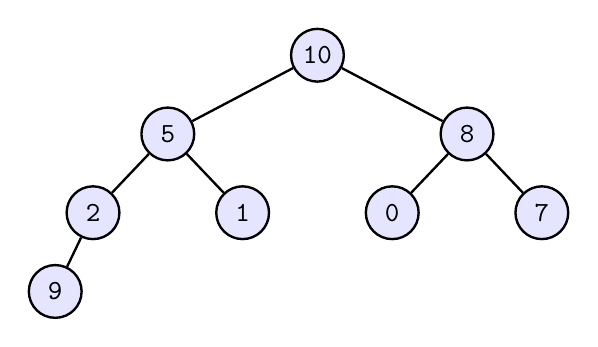
\begin{tikzpicture}

\fill[blue!10] (0.0, 0.0) circle (0.35);
\node [line width=0.03cm,black,minimum size=0.6699999999999999cm,draw,circle] at (0.0,0.0)(10){};\draw (0.0, 0.0) node[color=black] {\texttt{10}};
\fill[blue!10] (-1.9, -1.0) circle (0.35);
\node [line width=0.03cm,black,minimum size=0.6699999999999999cm,draw,circle] at (-1.9,-1.0)(5){};\draw (-1.9, -1.0) node[color=black] {\texttt{5}};
\fill[blue!10] (1.9, -1.0) circle (0.35);
\node [line width=0.03cm,black,minimum size=0.6699999999999999cm,draw,circle] at (1.9,-1.0)(8){};\draw (1.9, -1.0) node[color=black] {\texttt{8}};
\fill[blue!10] (-2.85, -2.0) circle (0.35);
\node [line width=0.03cm,black,minimum size=0.6699999999999999cm,draw,circle] at (-2.85,-2.0)(2){};\draw (-2.85, -2.0) node[color=black] {\texttt{2}};
\fill[blue!10] (-0.95, -2.0) circle (0.35);
\node [line width=0.03cm,black,minimum size=0.6699999999999999cm,draw,circle] at (-0.95,-2.0)(1){};\draw (-0.95, -2.0) node[color=black] {\texttt{1}};
\fill[blue!10] (0.95, -2.0) circle (0.35);
\node [line width=0.03cm,black,minimum size=0.6699999999999999cm,draw,circle] at (0.95,-2.0)(0){};\draw (0.95, -2.0) node[color=black] {\texttt{0}};
\fill[blue!10] (2.85, -2.0) circle (0.35);
\node [line width=0.03cm,black,minimum size=0.6699999999999999cm,draw,circle] at (2.85,-2.0)(7){};\draw (2.85, -2.0) node[color=black] {\texttt{7}};
\fill[blue!10] (-3.33, -3.0) circle (0.35);
\node [line width=0.03cm,black,minimum size=0.6699999999999999cm,draw,circle] at (-3.33,-3.0)(9){};\draw (-3.33, -3.0) node[color=black] {\texttt{9}};\draw[line width=0.03cm,black] (10) to  (5);
\draw[line width=0.03cm,black] (10) to  (8);
\draw[line width=0.03cm,black] (5) to  (2);
\draw[line width=0.03cm,black] (5) to  (1);
\draw[line width=0.03cm,black] (8) to  (0);
\draw[line width=0.03cm,black] (8) to  (7);
\draw[line width=0.03cm,black] (2) to  (9);
\end{tikzpicture}

\end{center}



It's easy to see that in the DFA, the $a$--
and $b$--transitions from the state $\{\}$ goes back to itself.
Therefore the completed DFA is this:


\begin{center}
\begin{tikzpicture}[>=triangle 60,shorten >=0.5pt,node distance=2cm,auto,initial text=, double distance=2pt]
\node[state,initial] (A) at (  0,  0) {$\{q_0\}$};
\node[state] (B) at (  3,  0) {$\{\}$};

\path[->]
(A) edge [bend left=0,pos=0.5,above] node {$a,b$} (B)
(B) edge [loop above] node {$a,b$} ()

;
\end{tikzpicture}
\end{center}
    



\newpage

Solution to Exercise \ref{ex:dfa-as-powerful-as-nfa1}\labeltext{}{sol:dfa-as-powerful-as-nfa1}.

\tinysidebar{\debug{exercises/{dfa-as-powerful-as-nfa1/answer.tex}}}

    Solution not provided.
    

\newpage

Solution to Exercise \ref{ex:dfa-as-powerful-as-nfa2}\labeltext{}{sol:dfa-as-powerful-as-nfa2}.

\tinysidebar{\debug{exercises/{dfa-as-powerful-as-nfa2/answer.tex}}}

    Solution not provided.
    

\newpage

Solution to Exercise \ref{ex:dfa-as-powerful-as-nfa3}\labeltext{}{sol:dfa-as-powerful-as-nfa3}.

\tinysidebar{\debug{exercises/{dfa-as-powerful-as-nfa3/answer.tex}}}

    Solution not provided.
    

\newpage

Solution to Exercise \ref{ex:dfa-as-powerful-as-nfa4}\labeltext{}{sol:dfa-as-powerful-as-nfa4}.

\tinysidebar{\debug{exercises/{dfa-as-powerful-as-nfa4/answer.tex}}}

    Solution not provided.
    

\newpage

Solution to Exercise \ref{ex:closure0}\labeltext{}{sol:closure0}.

\tinysidebar{\debug{exercises/{closure0/answer.tex}}}

    Solution not provided.
    

\newpage

Solution to Exercise \ref{ex:closure1}\labeltext{}{sol:closure1}.

\tinysidebar{\debug{exercises/{closure1/answer.tex}}}

    Solution not provided.
    

\newpage

Solution to Exercise \ref{ex:closure2}\labeltext{}{sol:closure2}.

\tinysidebar{\debug{exercises/{closure2/answer.tex}}}

    Solution not provided.
    

\newpage

Solution to Exercise \ref{ex:closure3}\labeltext{}{sol:closure3}.

\tinysidebar{\debug{exercises/{closure3/answer.tex}}}

    Solution not provided.
    

\newpage

Solution to Exercise \ref{ex:closure4}\labeltext{}{sol:closure4}.

\tinysidebar{\debug{exercises/{closure4/answer.tex}}}

    Solution not provided.
    

\newpage

Solution to Exercise \ref{ex:closure5}\labeltext{}{sol:closure5}.

\tinysidebar{\debug{exercises/{closure5/answer.tex}}}

    Solution not provided.
    

\newpage

Solution to Exercise \ref{ex:closure6}\labeltext{}{sol:closure6}.

\tinysidebar{\debug{exercises/{closure6/answer.tex}}}

    Solution not provided.
    

\newpage

Solution to Exercise \ref{ex:closure7}\labeltext{}{sol:closure7}.

\tinysidebar{\debug{exercises/{closure7/answer.tex}}}

    Solution not provided.
    

\newpage

Solution to Exercise \ref{ex:closure8}\labeltext{}{sol:closure8}.

\tinysidebar{\debug{exercises/{closure8/answer.tex}}}

    Solution not provided.
    

\newpage

Solution to Exercise \ref{ex:closure9}\labeltext{}{sol:closure9}.

\tinysidebar{\debug{exercises/{closure9/answer.tex}}}

    Solution not provided.
    

\newpage

Solution to Exercise \ref{ex:closure10}\labeltext{}{sol:closure10}.

\tinysidebar{\debug{exercises/{closure10/answer.tex}}}

    Solution not provided.
    

\newpage

Solution to Exercise \ref{ex:closure11}\labeltext{}{sol:closure11}.

\tinysidebar{\debug{exercises/{closure11/answer.tex}}}

    Solution not provided.
    

\newpage

Solution to Exercise \ref{ex:closure12}\labeltext{}{sol:closure12}.

\tinysidebar{\debug{exercises/{closure12/answer.tex}}}

    Solution not provided.
    
 % input solutions.tex
